\documentclass[tikz,border=10pt]{standalone}
\usepackage{tikz}
\begin{document}

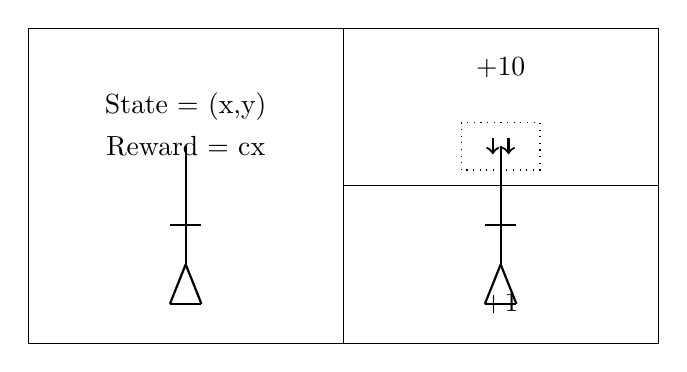
\begin{tikzpicture}

% Left box
\draw (0,0) rectangle (4,4);
\node at (2,3) {State = (x,y)};
\node at (2,2.5) {Reward = cx};
\draw[thick] (2,1.5) -- (2,2.5);
\draw[thick] (1.8,1.5) -- (2.2,1.5);
\draw[thick] (2,1) -- (2,1.5);
\draw[thick] (1.8,0.5) -- (2.2,0.5);
\draw[thick] (2,1) -- (1.8,0.5);
\draw[thick] (2,1) -- (2.2,0.5);

% Right box
\draw (4,0) rectangle (8,4);
\node at (6,3.5) {+10};
\node at (6,0.5) {+1};
\draw (4,2) -- (8,2);
\draw[thick] (6,1.5) -- (6,2.5);
\draw[thick] (5.8,1.5) -- (6.2,1.5);
\draw[thick] (6,1) -- (6,1.5);
\draw[thick] (5.8,0.5) -- (6.2,0.5);
\draw[thick] (6,1) -- (5.8,0.5);
\draw[thick] (6,1) -- (6.2,0.5);

% Treadmill arrows
\draw[dotted] (5.5,2.2) rectangle (6.5,2.8);
\draw[thick,->] (5.9,2.6) -- (5.9,2.4);
\draw[thick,->] (6.1,2.6) -- (6.1,2.4);

\end{tikzpicture}

\end{document}